%************************************************
\chapter{Evaluation and results}\label{cap:eval_and_res}
%************************************************

% switch between these depending on page size, or modify directly
% same for the rest of the chapters
\tikz[remember picture,overlay] \node[opacity=1,inner sep=0pt] at (current page.center){\includegraphics[width=\paperwidth,height=\paperheight]{./Figures/cover/firstshot_title.png}};
%\tikz[remember picture,overlay] \node[opacity=0.3,inner sep=0pt] at ([yshift=3cm,xshift=2cm]current page.center){\includegraphics[width=\paperwidth,height=\paperheight]{./Figures/cover/sesshu_1.jpg}};
\clearpage 

Lorem ipsu

\section{Scenario design}\label{sec:scenario_design}

Fusilar este paper!!!~\cite{Ostendorf2025} si no es bueno, mirar en arxiv con same name

The area chosen for the simulation scenarios is the city of Copenhagen, Denmark
Name kbh


decir q empezamos con secc tocha de la cual se recortaron la j1 etc para single int, corridor y network

\subsection{Road network generation}
\subsubsection{Definition}


The network scenario is defined geographically as the rectangular area delimited by the following thoroughfares: in the northeast, the Sølvgade-Fredensgade axis; in the northwest, the Blegdamsvej-Fælledvej-Blågardsgade direction; southwesterly the Åboulevard-Gyldenløvesgade-H. C. Andersens Boulevard; and southeasterly by the Nørre Voldgade-Øster Voldgade streets. The area contains dozens of intersections, of which 25 are signalized. Figure \ref{fig:area_sat} displays the area of interest along with the signalized junctions, oriented north.

\begin{figure}[h]
\centering
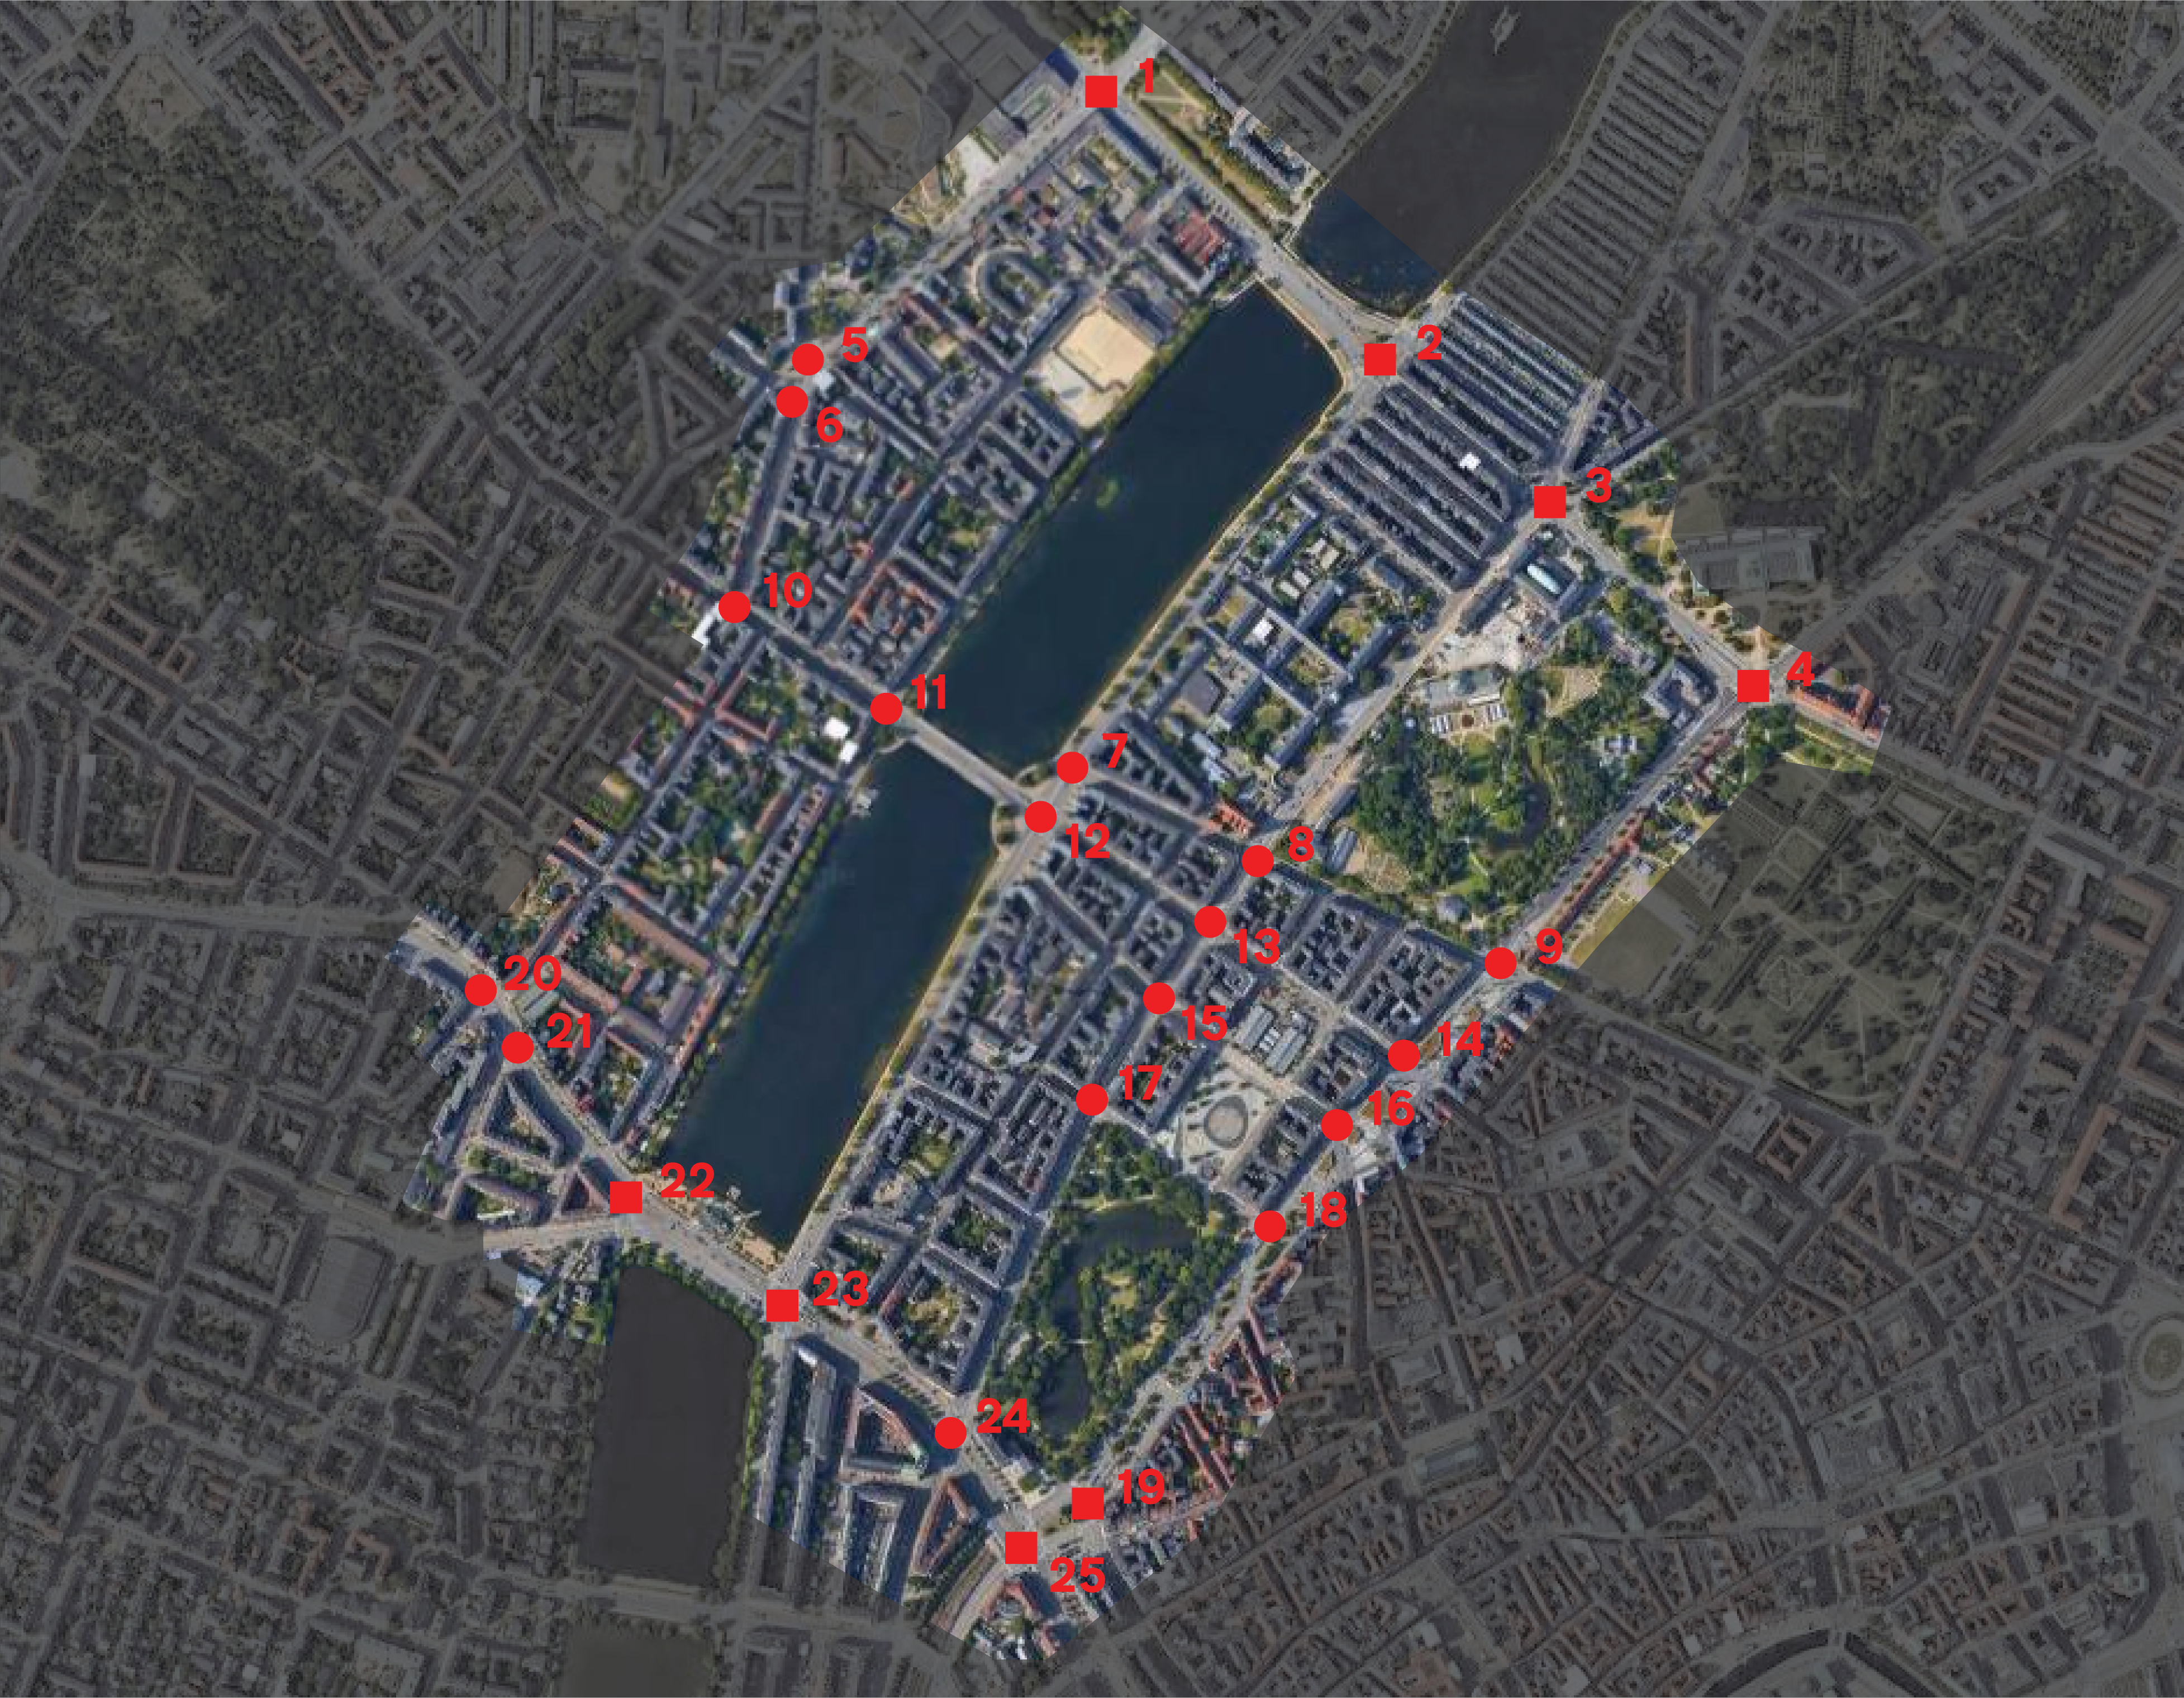
\includegraphics[width=0.8\linewidth]{Figures/chapter04/area_sat.png}
\caption[A satellite image of Copenhagen, Denmark, highlighting the network scenario area.]{A satellite image of Copenhagen, Denmark, highlighting the network scenario area. The red markers correspond to the signalized intersections, being round for conventional ones and square for compound ones. \textit{CNES, Airbus, Maxar Technologies}}
\label{fig:area_sat}
\end{figure}

This particular portion of Copenhagen was selected for its representativeness of the complexity of an actual urban environment with multimodal traffic. It includes streets with high traffic volumes for cars, like Åboulevard, while also for cyclist and pedestrians, as it encompasses the bustling Nørrebrogade thoroughfare, the street with the largest volume of cyclists in the city, all along until reaching the multimodal transit hub of the Nørreport station, the busiest in Denmark~\cite{norreport}. Furthermore, its position in the edges of the old city makes it boast a road network of significant sophistication, with special lanes, compound intersections and a great diversity of street types.

From the defined network, smaller portions were extracted to create the single intersection and corridor scenarios.

\medskip

\noindent \textbf{Single intersection}

\noindent For the single intersection scenario, the Tagensvej-Blegdamsvej-Fredensgade intersection —from now on, «J1»— was selected. Between through lanes and turn ones, J1 has three to four lanes on each approaching leg, and one to two of the ones coming out of it. All its approaches have sidewalks, dedicated or shared bike lanes and have pedestrians crossings across.

This intersection was chosen for its representativeness of a typical urban intersection in Copenhagen with multimodal traffic, with specific turn lanes, dedicated lanes for cyclists, and pedestrian crossings both with and without traffic islands.

It should be noted that the J1 intersection is a compound one, according to the the definition laid out in Section~\ref{subsubsec:intersections}. The intersection is composed of two subintersections, one for the main junction between the four streets, and another for the crossing of bike and pedestrian movements across the right-turn lane used for the car movement from Blegdamsvej to Tagensvej. See Figure~\ref{fig:j1_sat} for a better view of the intersection morphology.

\begin{figure}[h]
\centering
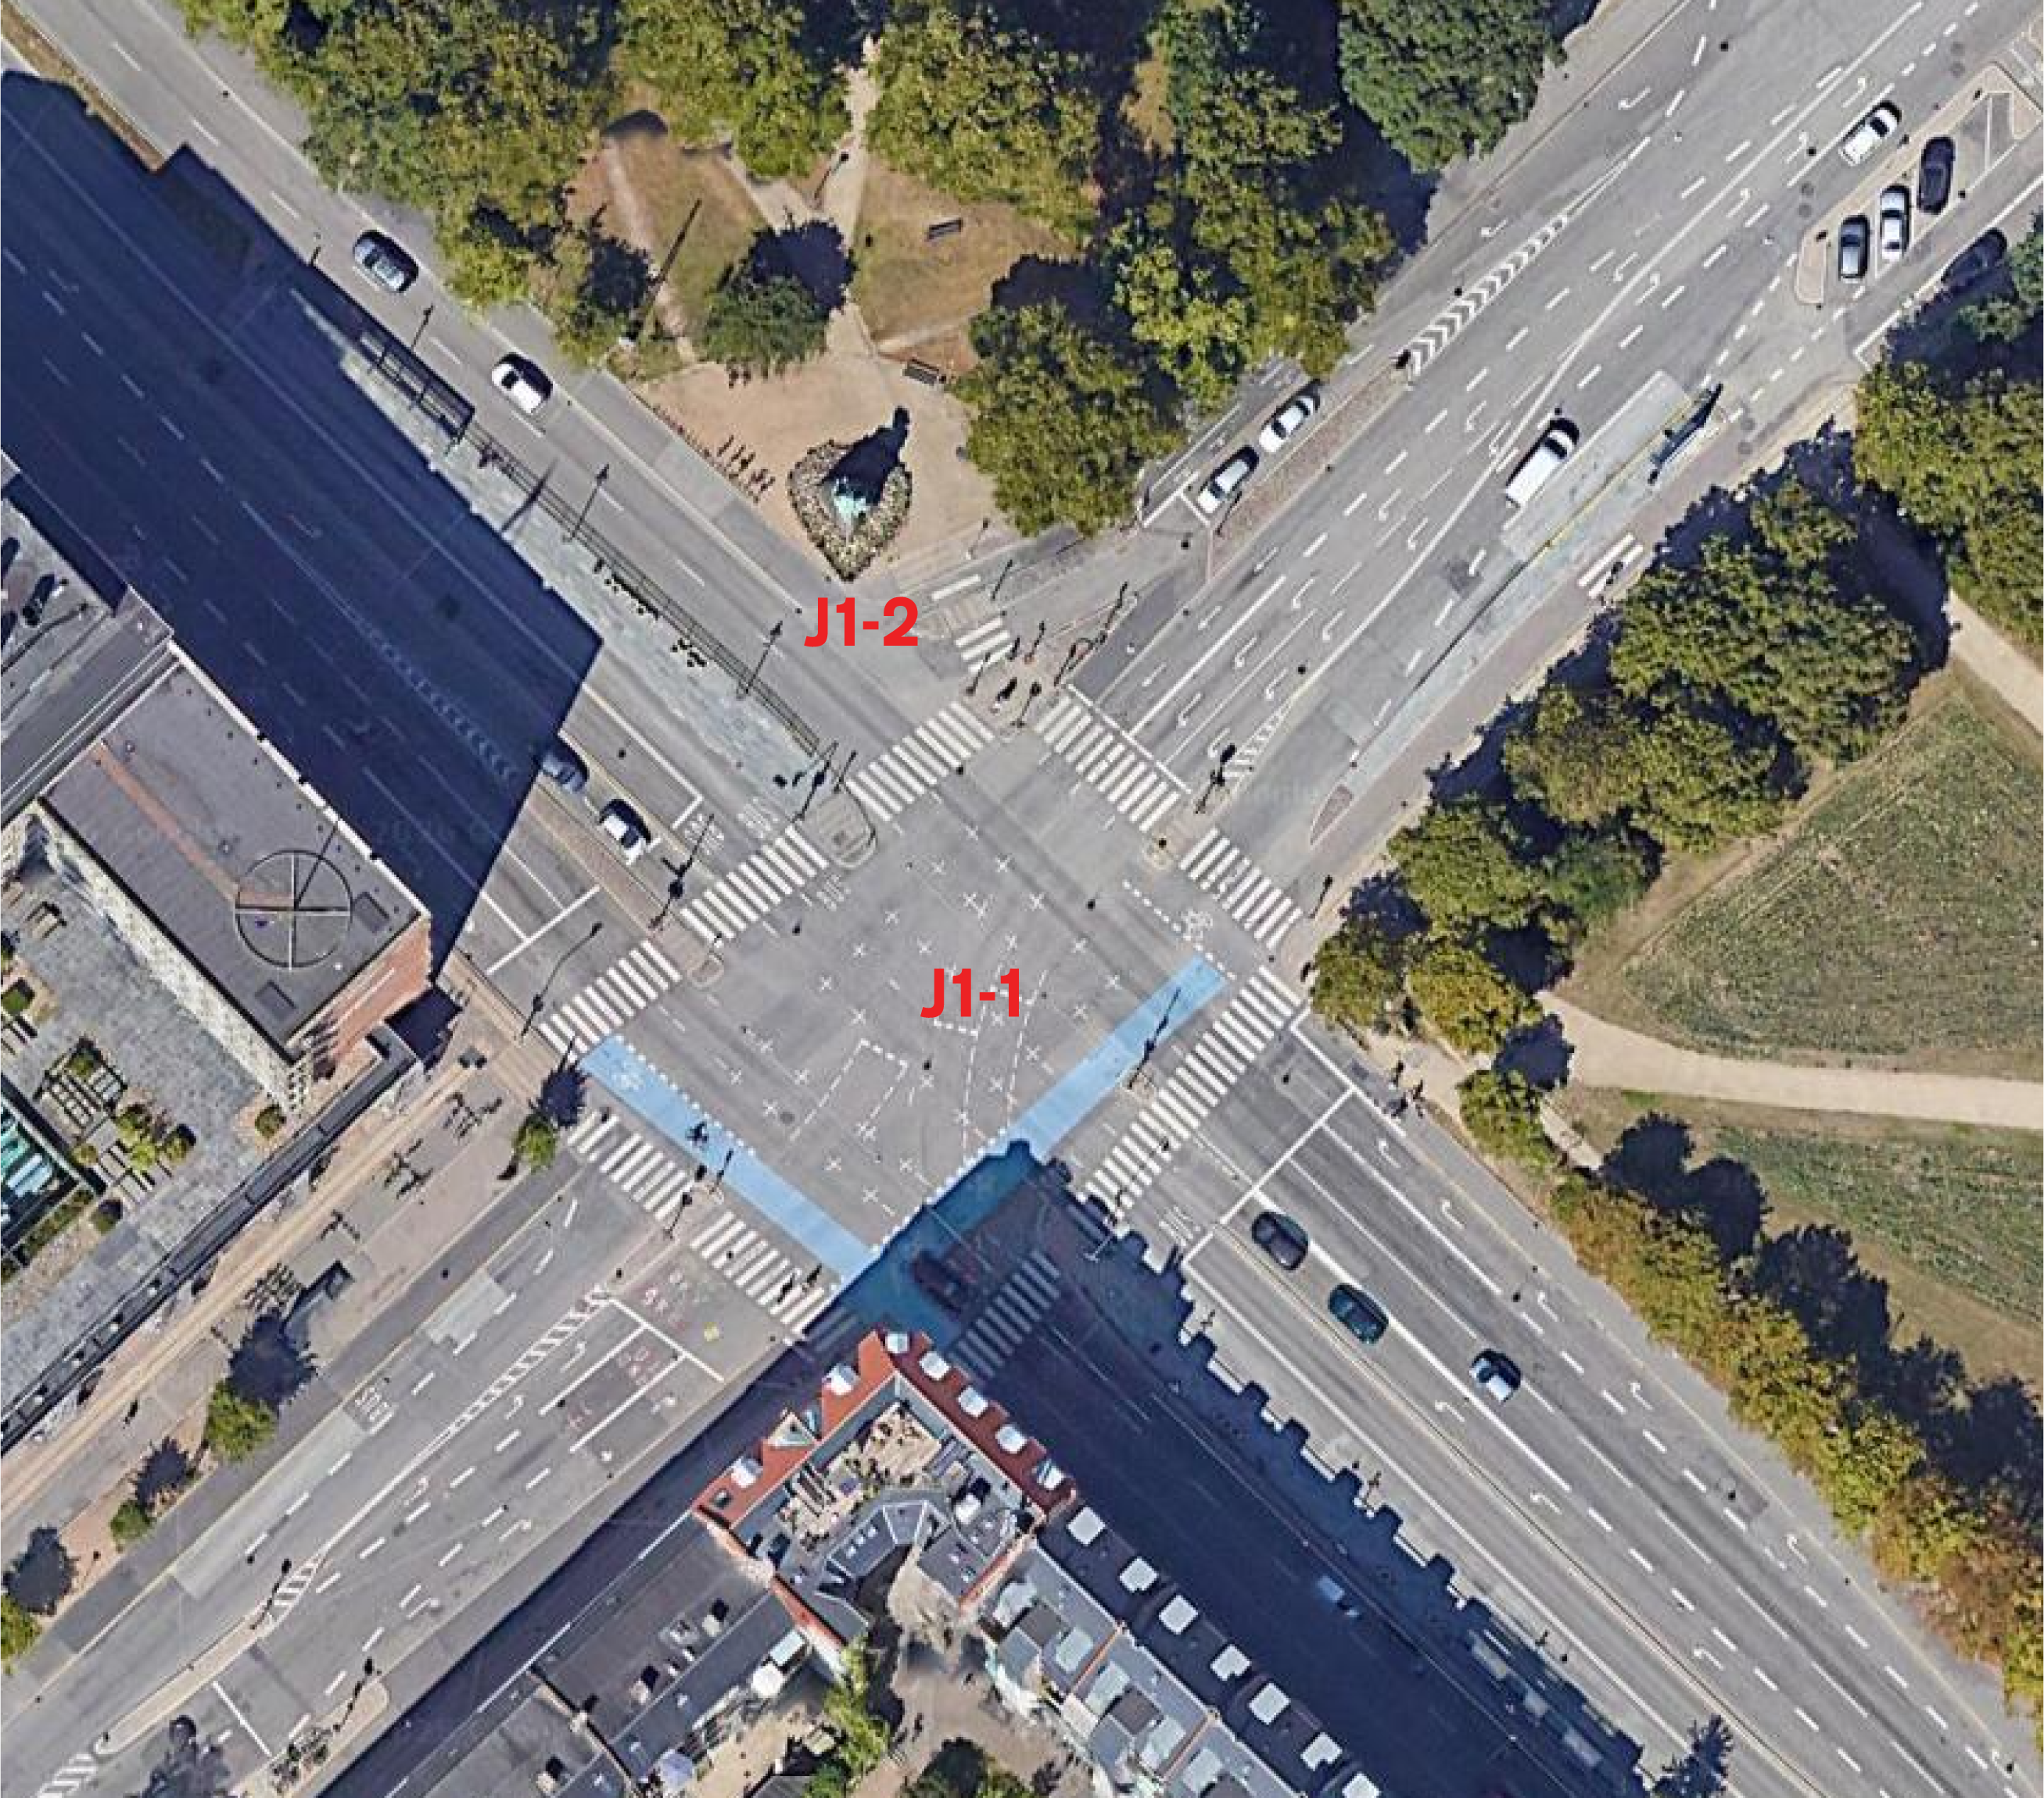
\includegraphics[width=0.8\linewidth]{Figures/chapter04/single_int_sat.png}
\caption[A satellite image of the J1 intersection.]{A satellite image of the J1 intersection.\protect\footnotemark~The image is oriented north, and the text indicates each subintersection. \textit{Airbus, Maxar Technologies}}
\label{fig:j1_sat}
\end{figure}

\footnotetext{For a different view, the photograph used for the chapter cover was shot by the author at this intersection.}

\medskip

\noindent \textbf{Corridor}

\noindent For the corridor scenario, the Frederiksborggade-Dronning Luises Bro-Nørrebrogade corridor —from now on, «C2»— was chosen, with five signalized intersections. Its streets have varying widths, ranging from a single lane on each direction to three when turn lanes are added before the intersections. All streets have sidewalks, dedicated bike lanes and occasionally bus lanes.

Its choice was also deliberate, as it contains Nørrebrogade, the street with the largest volumes of bicycle and pedestrian traffic, and finishes in the old city, just after the public transport hub of the Nørreport Station.

See Figure~\ref{fig:c2_sat} for a bird's-eye view of the corridor.

\begin{figure}[h]
\centering
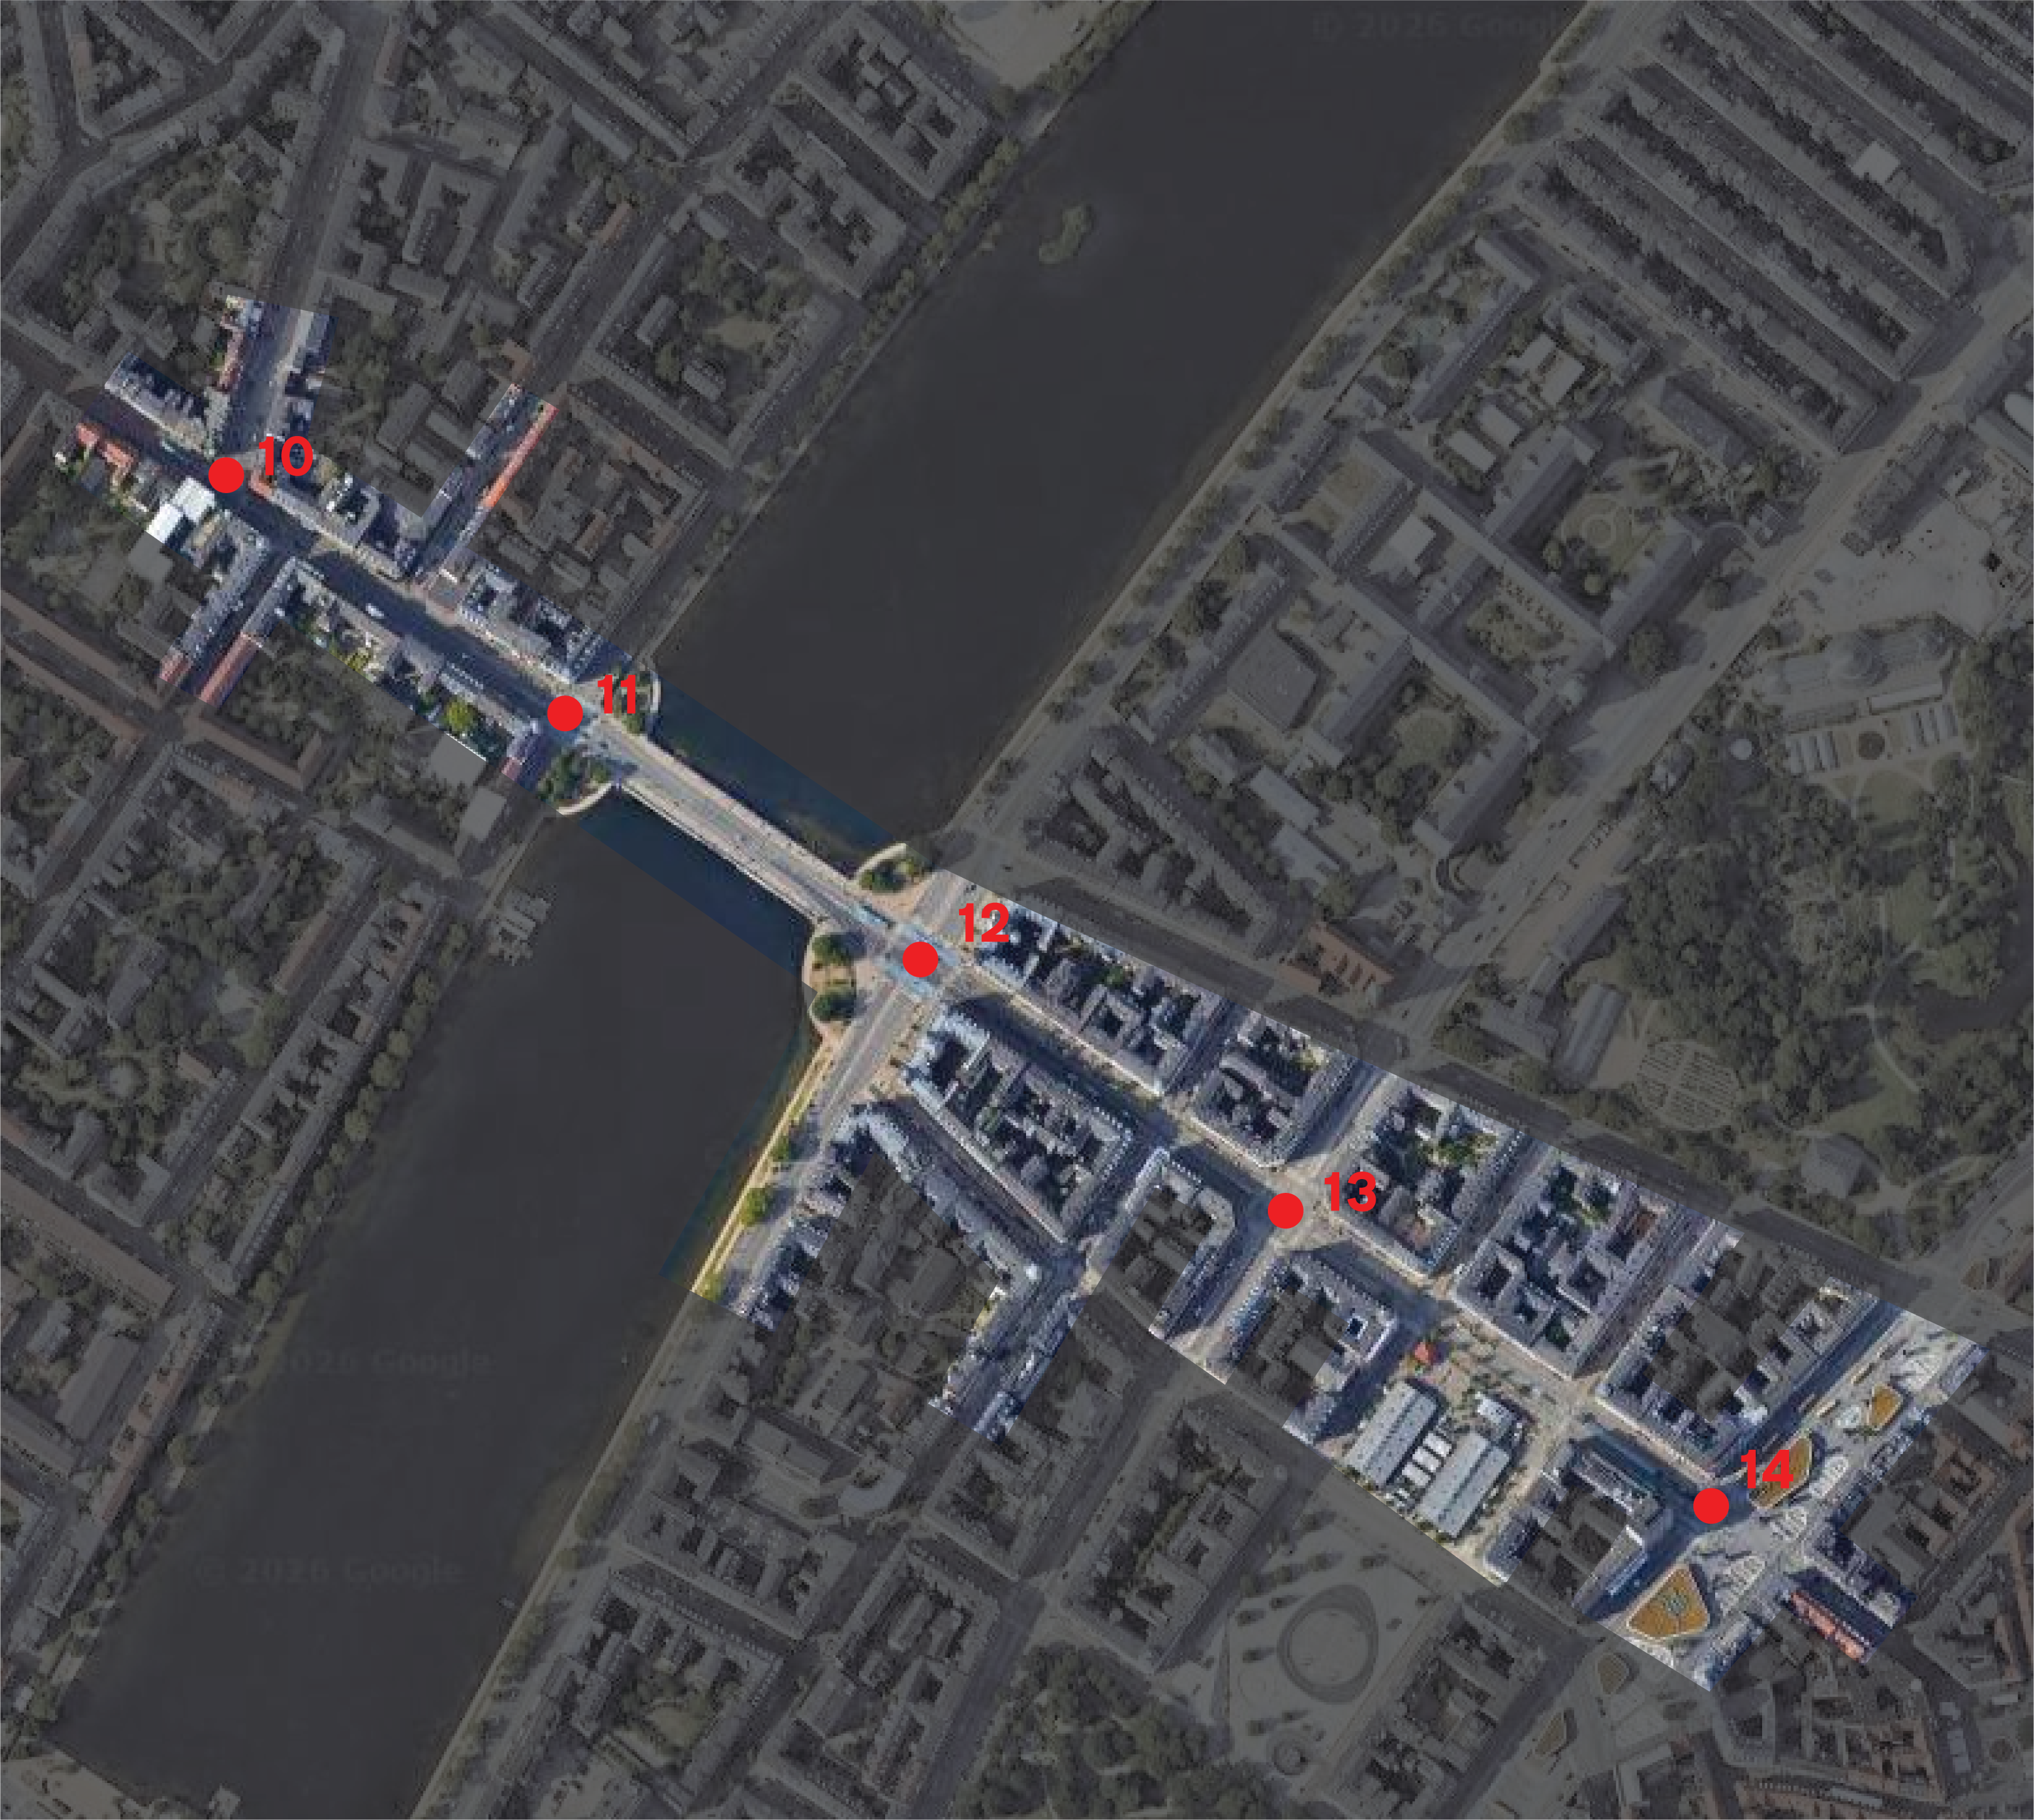
\includegraphics[width=0.8\linewidth]{Figures/chapter04/corridor_sat.png}
\caption[A satellite image of the corridor scenario.]{A satellite image of the corridor scenario. The markers follow the convention of those of Figure~\ref{fig:area_sat}. \textit{Airbus, Maxar Technologies}}
\label{fig:c2_sat}
\end{figure}


\subsubsection{Processing}

SUMO offers a tool named \texttt{netconvert} which can import road and street networks from different sources and convert them into compatible \texttt{.net.xml} files for their usage as SUMO networks.

OpenStreetMap is a collaborative map database maintained by volunteers that offers freely the download of street networks. We used its Overpass API to download the street network for the relevant area, using it as input for \texttt{netconvert}. However, the resulting network was not completely accurate, especially regarding intersections.

It was required to manually adjust the output to ensure proper representation of the streets, intersections, and their traffic signal configurations. To do so, we compared each lane and intersection in the network with satellite images, manually rectifying them using SUMO's \texttt{netedit} tool. \texttt{netedit} is a program developed by the SUMO team to edit SUMO networks using a GUI along with a wide range of capabilities.

Among the changes made across the network, many sub-intersections were needed to be merged into a single compound one, as Figure~\ref{fig:arreglos_ints} shows, which unfortunately disrupted any preexisting traffic signal cycles defined during the import process.

\begin{figure}[h]
\centering
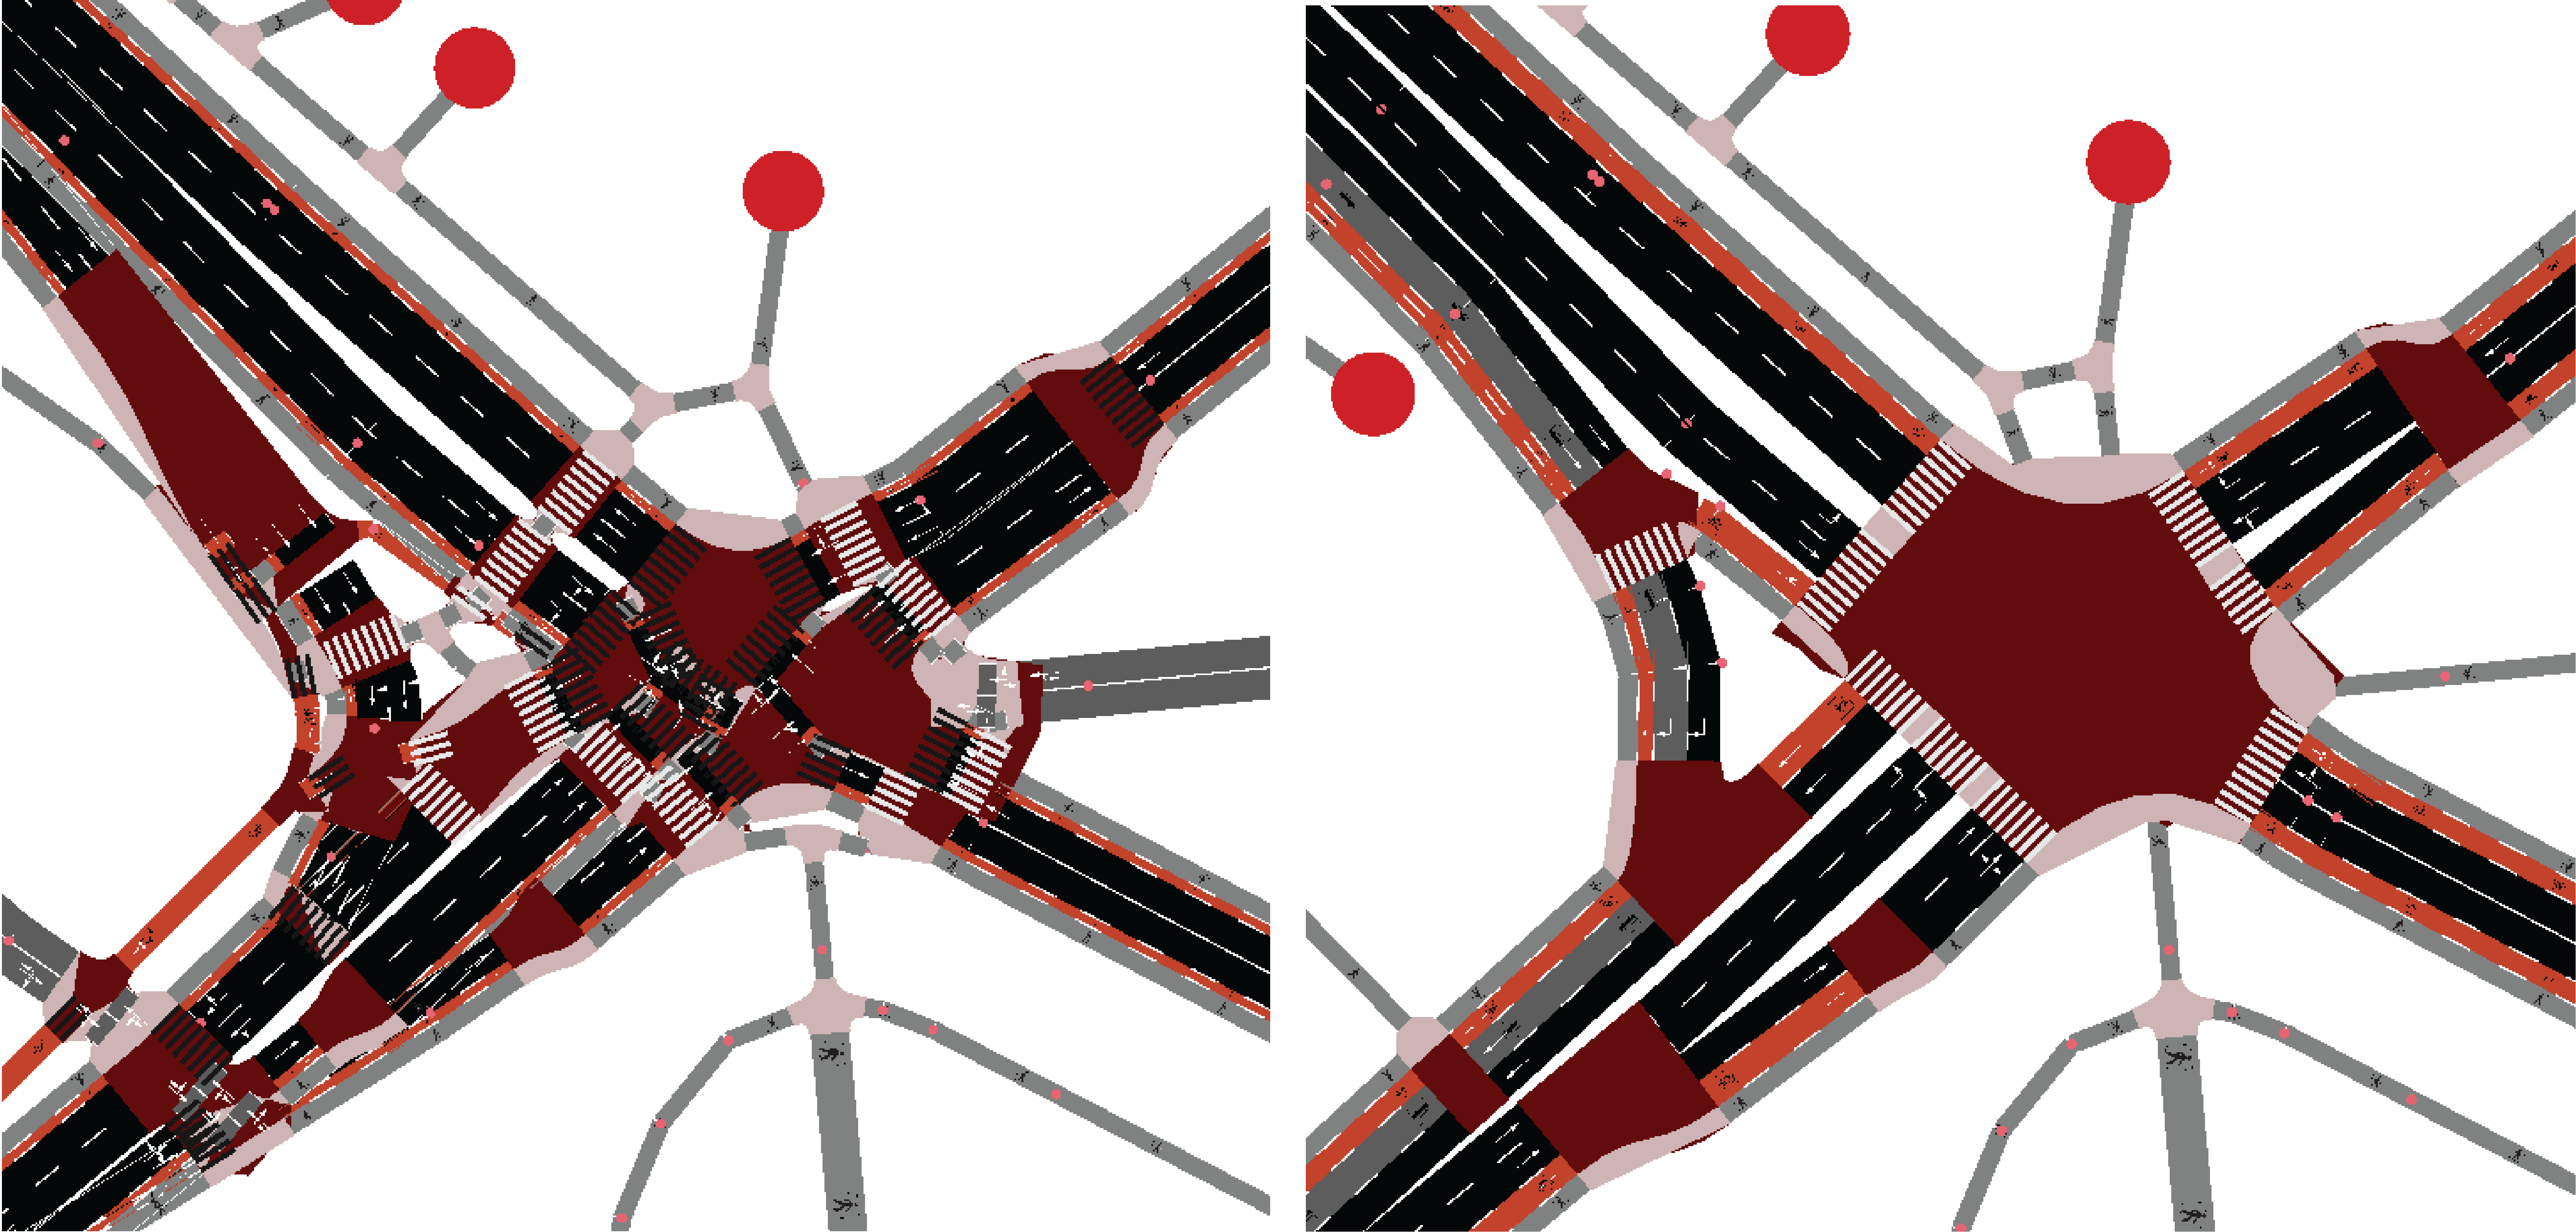
\includegraphics[width=0.8\linewidth]{Figures/chapter04/fixes.png}
\caption[Intersection exported from OpenStreetMap before and after manual corrections.]{Intersection exported from OpenStreetMap before and after manual corrections.}
\label{fig:arreglos_ints}
\end{figure}

To overcome this, the 25 signalized intersections were given movement and phase definitions manually. While this process was performed examining images from Google Street View —particularly for turning movements— and using engineering judgement, a majority of these movements and phases correspond to derivates of the standard configuration described in Figure~\ref{fig:fase_def}. 

\begin{figure}[h]
\centering

\includegraphics[width=0.5\linewidth]{Figures/chapter04/fases sems.png}
\caption[Typical movement and phase definition for a 4-way intersection.]{Typical movement and phase definition for a 4-way intersection.}
\label{fig:fase_def}
\end{figure}

Additionally, further changes to intersections were needed to represent what is known as the \textit{Copenhagen left} for cyclist left turn movements. This is a manoeuvre in which left-turning cyclists are required to go straight along with through automobiles from the same approach, stop at the other side, wait for the green interval for the cross street, and then continue straight to the cross street to finish the manoeuvre, in the shape of a letter «L» \cite{Chen2014}. As these turns are mandatory for cyclists in Denmark \cite{copenleft}, real bike traffic in Copenhagen follows this practice and the city's intersections are built for it, with holding areas for awaiting bikes and traffic signal phasing that considers these two-step movements. Hence, it was a requisite to also ensure that the simulated cyclists turn according to the real-world behaviour.
To represent this manoeuvre, several operations need to be performed for each and every left turn bike movement inside \texttt{netedit}. As this process was not found documented in the literature, instructions are provided so that it can help any reader wishing to create SUMO networks with Copenhagen lefts. Please note that this explanation refers to \texttt{netedit} version 1.25.0. First, the \textit{Connection mode} of \texttt{netedit} shall be entered, in order to show the different connections corresponding to movements in each intersection. Once in it, the relevant bike left movement —probably diagonal— has to be selected with a right click, and the option «Add to selected» chosen in the pop-up menu. With the relevant movement selected, the \texttt{netedit} mode needs to be switched to \textit{Inspect mode}, where a left click in the connection will show its attributes in the left pane. There, the «indirect» checkbox must be activated, which enables the option «Set custom connection shape» when right-clicking the connection. Then, the connection can be modified so that it follows the «L» shape that corresponds to the Copenhagen left, and if it is a shared lane, the vehicle permissions updated to only allow bicycles. Once this is done, the last step is to set the attribute «contPos» in the \textit{Inspect mode} left pane to define the position where the bikes will wait before the second step. The value to be introduced is as metres, counted from the connection start. It is important that, if the intersections is signalized, the priority of this modified movement during green phases is set to «Green-Minor», so that the left-turning bikes yield correctly to straight movements.

\begin{figure}[h]
\centering
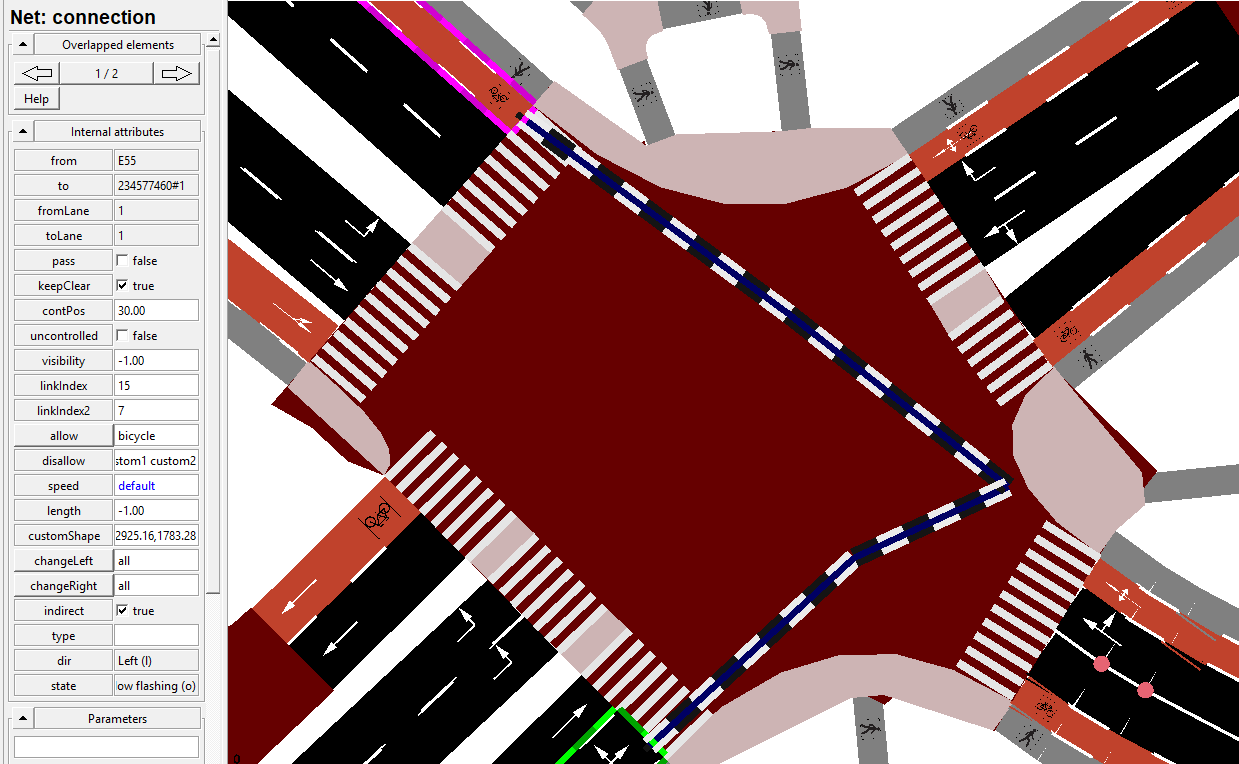
\includegraphics[width=0.8\linewidth]{Figures/chapter04/indirect turn setup.png}
\caption[Setup in \texttt{netedit} of a Copenhagen left.]{Setup in \texttt{netedit} of a Copenhagen left. Note on the left the attributes of the indirect connection.}
\label{fig:setup_indirect}
\end{figure}

The changes did not limit to intersections only. Again with the help of satellite imagery, bike lanes were added in streets that lacked them and removed from those that did not have them; bike lane widths were increased in streets across the network to correspond to their actual counterparts on the real world; vehicle permissions were adjusted in all the minor streets in the network that allow the roadway to be shared between modes; in the numerous streets that allow cyclists to ride in both directions while cars only have one, contraflow bike lanes were established to represent this configuration; bus lanes were defined where missing and, as also can be seen in Figure~\ref{fig:arreglos_ints}, turn lanes shared with cars on where created in all the intersections requiring.

\begin{figure}[h]
\centering
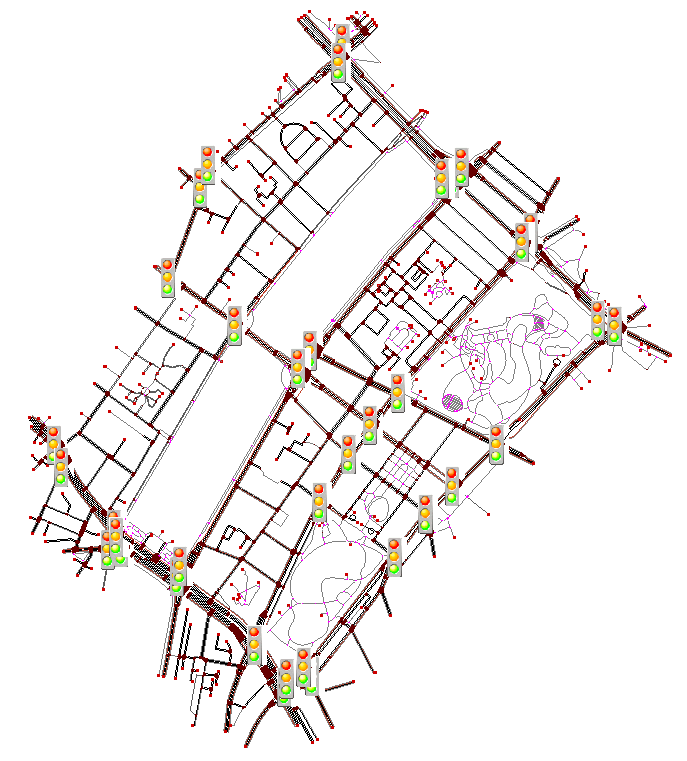
\includegraphics[width=0.8\linewidth]{Figures/chapter04/net_sumo.png}
\caption[The network scenario as seen in SUMO \texttt{netedit} after the necessary processing.]{The network scenario as seen in SUMO \texttt{netedit} after the necessary processing.}
\label{fig:net_sumo}
\end{figure}

\begin{figure}[h]
\centering
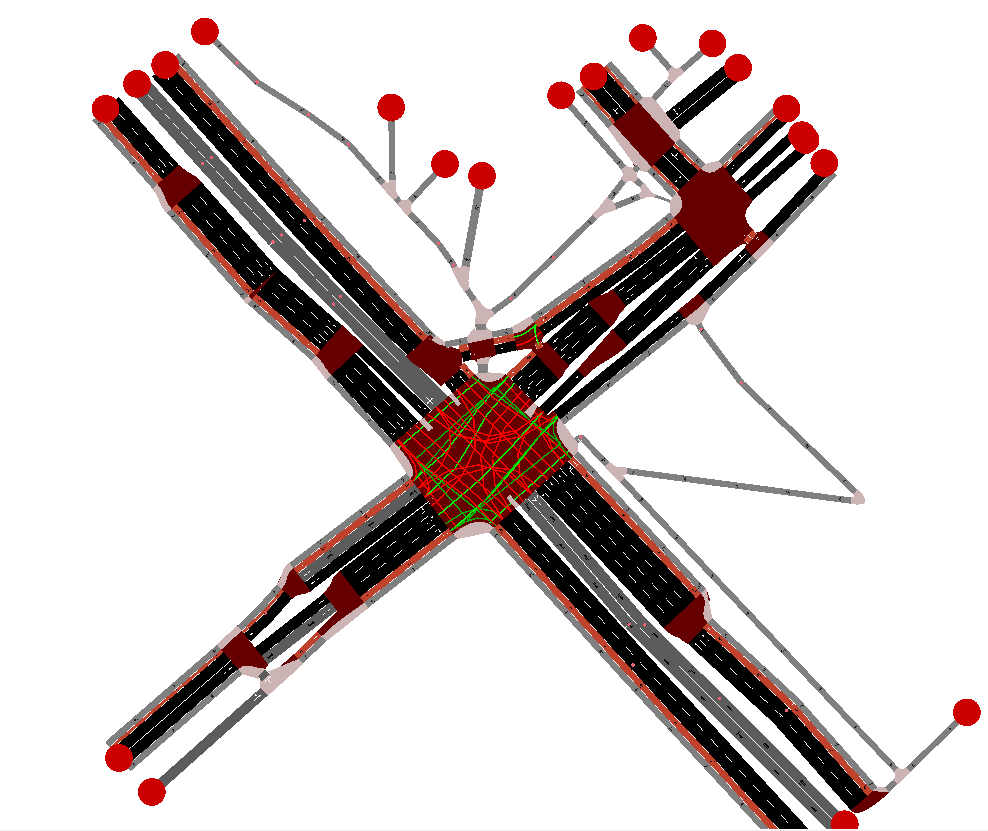
\includegraphics[width=0.8\linewidth]{Figures/chapter04/j1_netedit.png}
\caption[The single intersection scenario as seen in SUMO \texttt{netedit} after the necessary processing.]{The single intersection scenario as seen in SUMO \texttt{netedit} after the necessary processing. The screenshot was taken in the traffic signal mode, displaying the movements of one of the defined phases with coloured lights according to their state.}
\label{fig:j1_netedit}
\end{figure}

\begin{figure}[h]
\centering
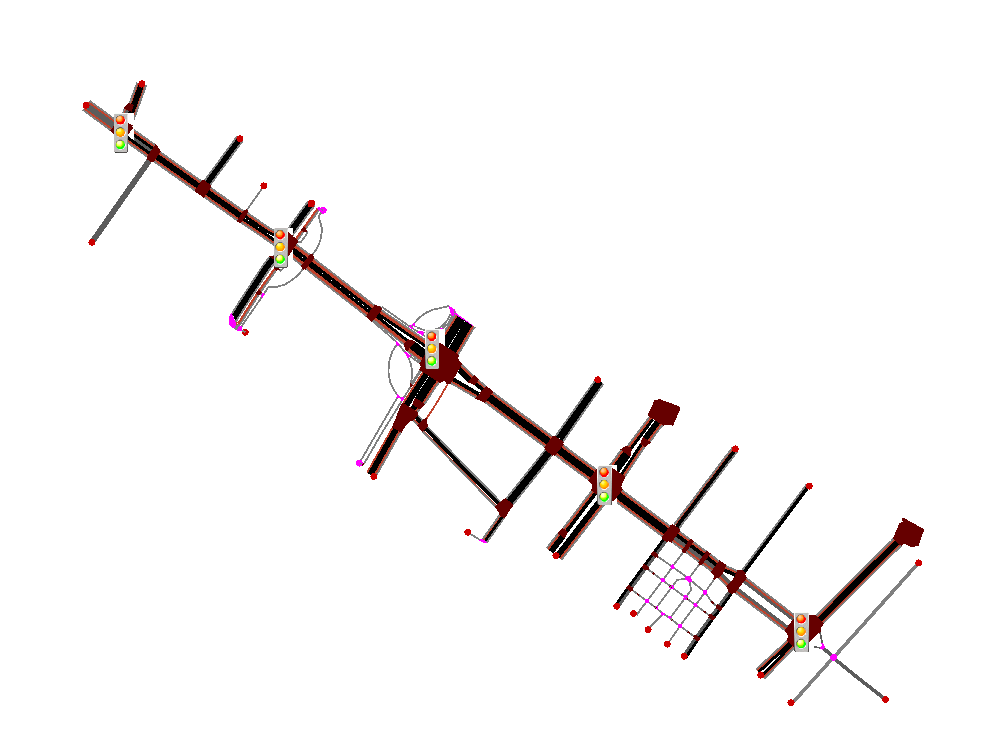
\includegraphics[width=0.8\linewidth]{Figures/chapter04/corridor_netedit.png}
\caption[The corridor scenario as seen in SUMO \texttt{netedit} after the necessary processing.]{The corridor scenario as seen in SUMO \texttt{netedit} after the necessary processing.}
\label{fig:c2_netedit}
\end{figure}

\subsection{Demand generation} \label{subsec:demand_generation}
\subsubsection{Data sources} 
Traffic count data was obtained from the COMPASS Copenhagen traffic model. COMPASS is a strategic, activity-based traffic model for the Greater Copenhagen area developed for the City of Copenhagen.\footnote{Further details about this model can be found in the presentation delivered by Paag \textit{et al.}~\cite{Paag2019}.} The data used corresponded to the model's base calculation for the year 2025, with 117\,558 link entries, of which 64\,071 were unique names, encompassing from pedestrian paths to motorways all throughout the Greater Copenhagen area.

COMPASS data is organized on a per-link basis, with entries for different stretches associated to geolocated polylines under EPSG:25832 (ETRS89, UTM zone 32N). Each entry has \gls{aadt} traffic count data for cars, bikes and pedestrians in both directions, along with average travel times in both directions for automobiles.

Figures \ref{fig:compass_car}, \ref{fig:compass_bike} and \ref{fig:compass_ped}, which can be examined in Appendix \ref{app:visual_compass}, show the COMPASS count data for the different modes in the area of interest.

\subsubsection{Demand modelling}

To generate SUMO demand from the data, the SUMO tool \texttt{routeSampler} was chosen.

This method is able to generate traffic demands based on turn count, edge count, and origin-destination count data, and is the only one of other available SUMO tools for this purpose that supports pedestrian routing. Furthermore, it is capable of handling routes with overlapping links and is the recommended option both in the SUMO documentation and the literature \cite{Ostendorf2025}.

As inputs, we provided 20\,000 possible routes in the network along with edge count and weight data to \texttt{routeSampler}, allowing the tool to select the appropriate distribution of routes to generate traffic demands reflecting the COMPASS data in the simulation.

To generate these possible input routes, two other SUMO tools were used in combination, \texttt{randomTrips} and \texttt{duarouter}, as suggested by the documentation and literature \cite{Ostendorf2025}.

For each mode, \texttt{randomTrips} generated the 20 000 random trips between points in the network, and these were converted with \texttt{duarouter} to valid routes by finding the shortest path fulfilling the trip.

Using SUMO definitions, a \textit{trip} is an origin-destination edge pair with a given departure time, without the edges between the points; while a \textit{route} is the valid set of edges that a specific entity actually travels from its generation to its removal from the simulation, generated from a trip, although several vehicles can have the same route. SUMO needs route files defining the movement of vehicles to be able to start a simulation.

The \texttt{randomTrips} module generates starting and destination points based on a defined distribution. To represent better the through traffic, its fringe factor parameter was increased to enlarge the probability of trips originating or ending on the scenario edges. With the generated trips, \texttt{duarouter} was then used to create routes based on them, using the Dijkstra shortest path algorithm \cite{Dijkstra1959}. Taking advantage of the average speed data for the car traffic, car edge weights were also given to \texttt{duarouter} in order to make route selection more realistic and related with the drivers' cost of time. The calculation of the aforementioned weights is explained along with the edge count data pairing, in the following paragraphs.

Besides the 20\,000 routes outputted by \texttt{duarouter}, \texttt{routeSampler}, we computed the edge counts and weights with a spatial matching procedure that transferred the COMPASS multimodal traffic volumes on an edge-to-edge basis to the SUMO network.

For each COMPASS link, the algorithm parsed the link's polyline geometry and reprojected it into the coordinate reference system of the SUMO network, applying a local offset to align it with SUMO's internal coordinate frame. A directional unit vector was computed from the polyline to characterize the link's orientation, and its reverse was also retained enabling the independent pairing to both traversal directions.

Because a single COMPASS dataset link may span multiple shorter SUMO edges (or viceversa), each link was discretized into a set of query points along its length: links under 30~m were represented by three points (start, midpoint, end), while longer ones were sampled at approximately 20~m intervals. For each query point and for each mode, the nearest candidate SUMO edges were identified from mode-specific spatial indexes —as SUMO edges' vehicle permissions can disallow some of the modes—, and a matching score combining directional cosine similarity and normalized distance was used to select the best-matching edge at that point. The union of best matches across all query points, for both the forward and reverse directions, constituted the set of matched SUMO edges for each COMPASS link and mode. If no match was found within the default search radius, the radius was expanded as a fallback before the link was marked unmatched.

The same pairing procedure was performed to the car durations reported for the SUMO links, in this case computing average car speeds for each matched car edge, derived from the COMPASS link's geometric length divided by the average reported travel time in each direction. These per-link speed estimates were aggregated across all COMPASS links mapping to a given SUMO edge using a flow-weighted average, yielding a single representative speed per SUMO edge which was the value used as weight in \texttt{duarouter}.

Once matched, the directional traffic volumes from the COMPASS dataset were assigned to the corresponding SUMO edges on a per-mode basis, scaled by mode-specific factors to convert average daily volumes into hourly flows. Every matched edge received the full volume for its direction, for it was assumed that any vehicle traversing the COMPASS link crosses each matched sub-edge in full. When only one direction yielded a match, that edge inherited the volume from both as a conservative compromise. Unlike car and bike lanes, sidewalks do not have a specific direction as pedestrian wander through them freely; to handle this circumstance, when matched sidewalk SUMO edges were found on both sides of a street, the total pedestrian volume in both directions was split evenly between the sides; if only one side had sidewalks, the full total was assigned to it.

\medskip

\noindent The mentioned factors used to compute hourly flows were calculated so that the assigned demand was that of a quarter of the peak hour demand.

It was the initial intention of this work to use the peak hour demand to represent the simulated scenarios under their worse conditions, however, hardware limitations made necessary to fraction the demand to one quarter of the intended values. The generated demand should then be understood as a realistic representation of off-peak hours Copenhagen traffic.

The obtention of the peak hour volumes from the \gls{aadt} count data was performed using a peak hour $k$ factor so that $\text{Peak hour volume} = k \cdot \text{\gls{aadt}}$.

The \gls{fhwa} states that in urban areas the $k$ value is placed towards the lower end of the $0.07-0.12$ range~\cite{FHWA2018}. To obtain a better estimate of the factor, the \gls{aadt} values for several locations obtained with COMPASS were assessed against the peak hours observed from actual count data for the same locations.\footnote{
        The counts assessed correspond to the ones reported in~\cite{kk_5},~\cite{kk_11},~\cite{kk_19},~\cite{kk_270},~\cite{kk_614},~\cite{kk_631},~\cite{kk_767}, ~\cite{kk_972},~\cite{kk_7005},~\cite{kk_7126},~\cite{kk_9691},~\cite{kk_9758},~\cite{kk_10259}, and~\cite{kk_Ny}.
} The $k$ factors found for each mode, and their corresponding fraction, are listed in Table \ref{tab:k_factors}.

\begin{table}[]
  \centering
\caption{$k$ factors and their corresponding fraction used for demand generation}
\label{tab:k_factors}
\begin{tabular}{lccc}
\hline
\multicolumn{1}{c}{\multirow{2}{*}{\textbf{Value}}} & \multicolumn{3}{c}{\textbf{Mode}}                   \\
\multicolumn{1}{c}{}                                & \textbf{Car} & \textbf{Bike} & \textbf{Pedestrians} \\ \hline
$k$                                                 & 0.0487       & 0.0844        & 0,0548               \\
\sfrac{1}{4}$k$                                     & 0.0122       & 0.0211        & 0.0137              
\end{tabular}
\end{table}

%\begin{equation}
    
%\end{equation}
  

\medskip

This process paired count data to 2817 edges in the SUMO network, and visual comparison proved a reasonable accuracy for the generated demand. The reader can compare the COMPASS data over a map of the relevant area with the generated demand in Appendix \ref{ch:app_gene}.

The procedure was performed on each of the scenarios, enabling in this way an accurate representation of the traffic from COMPASS data into all the SUMO simulations performed.

% DECIR Q NETWORK no tiene cruces de peatones mas q los pintaos pero q en calles interiores peatones cruzan a su bola y dificil modelar

% decir q hemos jutnado intersecciones proximas con semaforos pareados en signal groups xq
%  si no los modelos se volvian locos q no haboa espacio para modelar bien etc vease results de idqn en 420
% decir q hemos diseñado fases en SUMO manualmente basadas en reales xq las por defecto volvian loco
% a modelo; en todas, giros a dchas de bicis estan en green minor para repre como ceden paso a peats

\section{Experiments}
\subsection{Experimental setup}

From the scenarios, a series of experiments was performed to assess the performance of the proposed model and understand better 

The experiments were performed in different workstations of varying equipment, depending on availability: AMD Threadripper 3970X with two Nvidia RTX 2080Ti, AMD Threadripper 3960X with two Nvidia RTX 3080Ti or Intel Core i7-13700H with a single Nvidia RTX 4080 Laptop.

decir cantidad de cada modo por exp

\subsection{Evaluation metrics}

Lorem ipsum

\section{Results}

Lorem ipsum